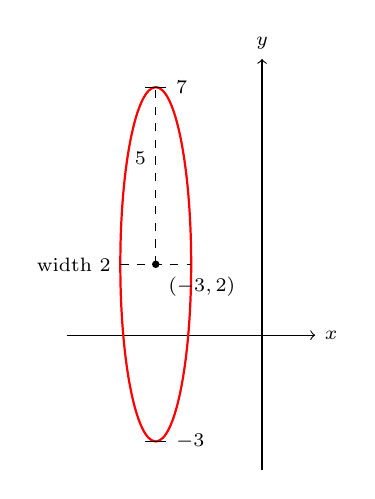
\begin{tikzpicture}[scale=0.45, every node/.style={font=\scriptsize}]
  \draw[->] (-5.5,0) -- (1.5,0) node[right] {$x$};
  \draw[->] (0,-3.8) -- (0,7.8) node[above] {$y$};
  \draw[red, thick] (-3,2) ellipse (1 and 5);
  \fill (-3,2) circle (3pt) node[below right=1pt] {$(-3,2)$};
  \draw[dashed] (-3,2) -- (-3,7) node[pos=0.6, left] {$5$};
  \draw[dashed] (-4,2) -- (-2,2);
  \node[below] at (-3,1.9) {};
  \draw (-3.3,7) -- (-2.7,7) node[right] {$7$};
  \draw (-3.3,-3) -- (-2.7,-3) node[right] {$-3$};
  \node[left] at (-4,2) {width $2$};
\end{tikzpicture}
